\documentclass[twoside,openright]{uva-bachelor-thesis}

\usepackage[utf8]{inputenc}
\usepackage{ae,aecompl}
\usepackage{sourcecodepro}
\usepackage[T1]{fontenc}

\usepackage{parskip}

\usepackage{lipsum}
\setlipsumdefault{131}

\usepackage{emptypage}

\usepackage[square,numbers]{natbib}
\usepackage[nottoc,numbib]{tocbibind}
\renewcommand\bibname{References}

\usepackage{graphicx}
\usepackage{epstopdf}
\usepackage{float}

\usepackage{hyperref}
\hypersetup{pdfborder={0 0 0}}

\setlength{\parindent}{0pt}
\setlength{\parskip}{1.3ex plus 0.5ex minus 0.3ex}

% Captions
\usepackage[format=plain,labelfont=sf,bf,up,textfont=it,up]{caption}
\usepackage{subfig}

% Code formatting
\usepackage{color}
\usepackage{listings}

\lstset{
	language=C++,                   % choose the language of the code
	basicstyle=\ttfamily\footnotesize, 		% the size of the fonts that are used for the code
	numbers=left,                   % where to put the line-numbers
	numberstyle=\footnotesize\color{gray},		% the size of the fonts that are used for the line-numbers
	stepnumber=1,                   % the step between two line-numbers. If it is 1 each line will be numbered
	numbersep=10pt,                  % how far the line-numbers are from the code
	showspaces=false,               % show spaces adding particular underscores
	showstringspaces=false,         % underline spaces within strings
	showtabs=false,                 % show tabs within strings adding particular underscores	
	frame=top, frame=bottom,        % adds a frame around the code
	xleftmargin=17pt,				% padding..
	framexleftmargin=17pt, framexrightmargin=17pt, framexbottommargin=5pt, framextopmargin=5pt,
	tabsize=2,          			% sets default tabsize to 2 spaces
	captionpos=t,           		% sets the caption-position to bottom
	breaklines=true,        		% sets automatic line breaking
	breakatwhitespace=true,    		% sets if automatic breaks should only happen at whitespace
	escapeinside={\%*}{*)},         % if you want to add a comment within your code
	morecomment=[l]{//}, 			% use comment-line-style!
	morecomment=[s]{/*}{*/}, 		% for multiline comments
	morekeywords={  abstract, event, new, struct,
		as, explicit, null, switch, base, extern, object, this,
		bool, false, operator, throw,
		break, finally, out, true, byte, fixed, override, try,
		case, float, params, typeof, catch, for, private, uint,
		char, foreach, protected, ulong, checked, goto, public, unchecked,
		class, if, readonly, unsafe, const, implicit, ref, ushort,
		continue, in, return, using, decimal, int, sbyte, virtual,
		default, interface, sealed, volatile, delegate, internal, short, void,
		do, is, sizeof, while, double, lock, stackalloc,
		else, long, static, enum, namespace, string},
}

\DeclareCaptionFormat{listing}{\rule{\dimexpr\textwidth+17pt\relax}{0.4pt}\par\vskip1pt#1#2#3}
\captionsetup[lstlisting]{format=listing,singlelinecheck=false,margin=0pt}
\renewcommand\lstlistingname{Snippet}
\newcommand{\includecode}[2]{\lstinputlisting[caption=#1]{samples/#2}}

% Other formatting.
\newcommand{\file}[1]{\texttt{#1}}
\newcommand{\code}[1]{\texttt{\footnotesize#1}}
\usepackage{verbatim}

\title{Modernizing the Civic \\compiler framework}
\author{Floris den Heijer\\5873355}
\supervisors{dr. C. Grelck}
\signedby{}

\begin{document}
\maketitle
\begin{abstract}
	\lipsum
\end{abstract}

\tableofcontents


\chapter{Introduction}
	\section{Problem Statement}
		Computer Science undergraduates at the University of Amsterdam have the option to learn the essentials of compiler construction by taking an eight week course where the main deliverable is a working compiler for a C-like educational language dubbed Civic. Construction of the compiler is assisted by a toolchain which consists of a custom virtual machine, assembler and development framework. In general, the course is received well and produces functional compilers. A recurrent issue however is the difficulty in getting up to speed with development, largely due to the technical challenges the chosen language (C99) poses and the lack of documentation for the framework.
		
		This paper will present an analysis of the compiler framework and the concepts on which it is based. A new framework is proposed which adapts these concepts and implements them in C\#, a modern managed language.
			
	\section{Context}
		Purpose of framework, teaching objectives, timeline.
		Other compiler frameworks, LVVM as backend, research on teaching methods for compiler construction??
		
		The Civic framework is used in a well-defined educational setting and as such omits many aspects of more advanced, general purpose compiler frameworks. Teaching objectives dictate the primary focus to be on the development of a fully functional frontend (scanning, parsing, semantic analysis), rather than a backend suited for heavy optimization.
		
		TODO
	
	\section{Objectives}
		The primary goal of this project is to analyze what a transition to an object-oriented language affects the Civic compiler framework. Key questions:
		\begin{itemize}
			\item Which concepts make the foundation of the current framework?
			\item Are these concepts implemented differently in a modern OO-language?
			\item What benefits might an OO-language add to the framework?
		\end{itemize}
		
		TODO
	
	\section{Research Approach}
		Analysis of existing framework, consideration of language dependent and independent factors, limitations of analysis.
		
		TODO
	
	\section{Scope And Limitations}
		 Focus is placed on creating a flexible abstract syntax tree which is suitable for basic optimization and code emission, eliminating the need for a seperate intermediate representation. While greatly simplifying the compiler pipeline, this reduces the framework to a near 'frontend-only' role and limits comparisons with other frameworks.
		
		This paper is limited to the compiler framework of the toolchain. This paper will not cover analysis of the Civic VM, assembler, teaching objectives or the suitability of alternative target languages such as LVVM, CIL or Java bytecode \cite{lattner2002llvm}\cite{website:sac}. Analysis of the existing framework is limited to the extraction of key concepts.


\chapter{Analysis Of Civic Framework}
	This chapter will provide an overview of the existing framework and it's conceptual foundation. On a high level the framework aims to provide a structured approach for phase-based transformations on a language agnostic AST. Central to the framework is the specification of the abstract syntax tree (AST) and a code generator which creates macro's to access these nodes from code, as well as traversal entry points and control mechanisms. Automatic traversals which copy, free or check a (sub-)tree are also generated.
	
	The Flex scanner generator and Bison parser generator is are integrated by default and a basic configuration is provided which allows parsing of a subset of the Civic expression language. In addition it generates documentation on the AST, provides a small base library for string manipulation, lookup tables and argument parsing and a testing suite.
				
	\section{Architecture}
		\begin{figure}[H]
			\centering
			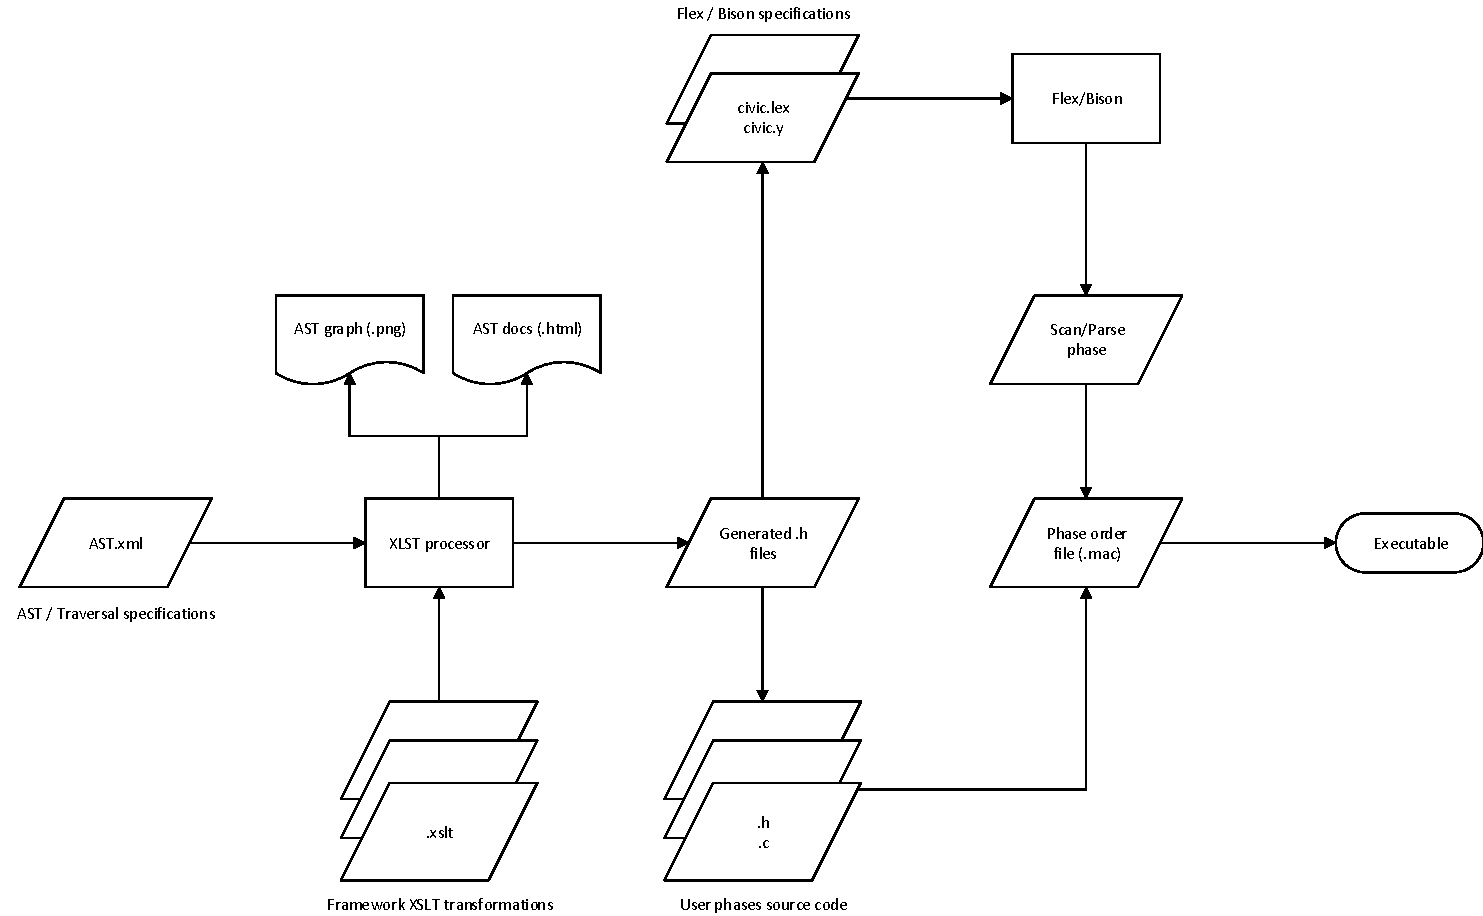
\includegraphics[width=0.95\textwidth]{figures/architecture/overview.pdf}
			\caption{Schematic overview of the Civic framework}
			\label{fig:build-dep}
		\end{figure}
	
		The framework is written in C and XLST and runs on most *nix distributions, provided they support the required packages \footnote{gcc, gzip, flex, bison, xsltproc, dot, indent}. A schematic overview of the architecture is presented in figure~\ref{fig:build-dep}. The framework relies on an XSLT processor to transform an AST and traveral specification into framework code used by the rest of the compiler. This process is triggered on each build and replaces key framework header files once the specifications are altered.
		
		User code is largely concentrated in AST transformations known as sub-phases, examples of which are type checking and context analysis. These sub-phases are grouped into logical phases, such as semantic analysis or code generation. Phases play a role in AST validation as described in section \ref{sec:validation} and are integrated into the command line, providing the option to only compile up to a certain phase, or output extra debug information during a phase. During the compilation of the compiler, phases are flattened into a sequence of traversals and control code is added which pipes the output of one traversal into the next.
		
		Names for library functions and phases adhere to an uppercase prefix followed by a lower camelcase identifier (\code{[PFX]someId}).
		
		
	\section{Code Generation From XML}
	\label{sec:old-sec}
			One defining characteristic of the framework is an abstraction layer over the AST and traversal mechanisms. To better understand this layer, this section will first summarize how nodes and traversals are internally represented, then detail how the abstraction assists in this process and conclude with a summation of all parts of the framework affected by the layer.
			
			Nodes are stored as a C-struct containing the type of the node and two structures representing their children and attributes (snippet \ref{old-arch:node}). For each node type there are two data structures with it's specific attributes and references to child nodes, the union of which is refered to in the \code{NODE} struct (snippet \ref{old-arch:union}). Access macro's are created for each attribute and child node as well as (de-)allocation code.
			
			\begin{lstlisting}[caption=Node structure,label=old-arch:node]
struct NODE {
	nodetype             nodetype;       /* type of node */
	int                  lineno;         /* line of definition */
	node*                error;          /* error node */
	struct SONUNION      sons;           /* child node structure */
	struct ATTRIBUNION   attribs;        /* attributes node structure */
};

typedef struct NODE node;
			\end{lstlisting}
			\begin{lstlisting}[caption=Sample child node and attribute union structures for node,label=old-arch:union]
struct SONS_N_VARDEC {
	node *Init;
};

struct ATTRIBS_N_VARDEC {
	char *Id;
	char *Type;
};

struct SONUNION {
	struct SONS_N_VARDEC *N_vardec;
	..
};

struct ATTRIBUNION {
	struct ATTRIBS_N_VARDEC *N_vardec;
	..
};
			\end{lstlisting}
			
			Traversals do not have a well defined single structure but translate into control flow statements and traverse tables. Users can push a traversal onto the stack and request the start of a traversal (snippet \ref{old-arch:start-trav}), triggering a lookup to a table for the active traversal holding the function which should be called index on node type. By default all child nodes are traversed using a switch statement based on node type (snippet \ref{old-arch:switch-trav}). The \code{INFO} struct passed along provides statefulness to receiving functions, though this is not essential for traversal.
			
			\begin{lstlisting}[caption=Starting a traversal,label=old-arch:start-trav]
node *n = ..;      /* retrieved elsewhere */
INFO *info = ..;   /* retrieved elsewhere */

TRAVpush(TR_mytrav);
n = TRAVdo(n, info);
TRAVpop();
			\end{lstlisting}
			\begin{lstlisting}[caption=Excerpt from catch-all switch construct,label=old-arch:switch-trav]
node *TRAVsons (node *arg_node, info *arg_info)
{
	switch (NODE_TYPE (arg_node)) {
		case N_program:
		TRAV (PROGRAM_DECLARATIONS (arg_node), arg_info);
		break;
		
		case N_declarations:
		TRAV (DECLARATIONS_DECLARATION (arg_node), arg_info);
		...
}
			\end{lstlisting}
						
			To illustrate the complexity involved, consider the introduction of a new node to the AST. To achieve this, every traverse table must be supplemented, the default traverse function must be updated, two new structures must be added to the node union, allocation and de-allocation routines must be written as well as access macro's and the copy, free and check system traversals must be modified. Besides being tedious, performing these tasks manually introduces a significant risk of error. The framework provides XSLT transformations of a specification to automate most of this process. It takes only a couple of lines of XML to add a node to the AST, and all previously mentioned tasks are automatically executed. This does however mean that the specification forming the abstraction is not isolated from the target language (or leaky). For instance, to define a node with a \code{char*} attribute requires the specification to know about the difference in copying C-strings and integers.
					
			Specifications and accompanying translations are given for:
			\begin{itemize}
				\item Nodes which form the abstract syntax tree, along with their applicable attributes and child nodes
				\item Mapping from friendly attribute names to C-types, and relevant methods used for copying and free-ing
				\item Node constraints on:
				\begin{itemize}
					\item Type: only certain child nodes or attribute are valid
					\item Requirement: attributes or child node must be present
					\item Applicable phase: some attributes are not always required
				\end{itemize}
				\item Traversals, their mode of operation, affected nodes and function prefix
			\end{itemize}
		
	\section{Flexible Traversals}
			Internals of the traversal have been briefly shown in section \ref{sec:old-sec} and will be explained in more detail in this section. 
			
			Traversals are supported in two modes: 1) user mode and 2) child mode. User mode traversals are required to implement handlers for every node type defined in the AST, child mode requires only handlers for a specified list of nodes. Every node which is not on the user specified list is routed instead to a catch-all function which automatically traverses child nodes of the unhandled node. This function is automatically updated when a node is added or removed or a change is made to any of the child node properties.
			
			All traversals are elements in the \code{<phases>} element of the specification document, and must contain a unique identifier, readable short name, operation mode (user or child), associated header file and - depending on the chosen mode - a list of nodes handled by the traversal. When the compiler is built, enumerations of all node and traversal identifiers are generated. All nodes and traversals are assigned a zero-indexed integer to be used as an index. Every traversal adds an array of function pointers to the traverse table. The row is added at the index dictated by the enumeration and the array is indexed by the node index. References to the funtions are constructed by concatenating the traversal identifier with the friendly name of the node. In child mode, unhandled node types are routed to the catch-all function explained in the last paragraph.
			
			Every handler has the same function signature, requiring pointers to a node and an info structure, and returning a pointer to a node which replaces the current node. If a traversal is to be used as an entry point for a sub-phase, it must be added to the \code{phase.mac} file, where an entry point is referenced with the same signature as a handler function: \\
			\code{node *PFXnodeType (node *arg\_node, info *arg\_info)}
						
			The framework maintains a stack of active traversals manipulated with the \code{TRAVpush (id)} and \code{TRAVpop ()} functions. An active traversal can be controlled with the \code{TRAVdo (node*, info*)}, \code{TRAVopt (node*, info*)} and \code{TRAVcont (node*, info*)} functions. All return the result of the traversal of a given subtree, additionally the latter two respectively ignore null node arguments and invoke the catch-all handler.
			
			This approach to traversals encourages users to create small, reusable traversals in similar way the visitor pattern is implemented in an object-oriented language \cite{gof1994}.
			
	\section{Tree Validation}\label{sec:validation}
			As explained in section \ref{sec:old-sec}, nodes all share the same structure. Semantically all node structures are valid trees, yet most combinations of AST nodes should yield an invalid tree. This section briefly explains the validation mechanisms present in the framework.
			
			The first line of defense against illegal node operations is the tagged union implemented for nodes. A tagged union is a structure which can take on different but fixed types \cite{unknown}. An \code{enum} is used to distinguish all different node types and used in the generated traversals to always pick the correct structure when traversing. Unlike  functional languages, C provides no compile time checks to enforce the tagged union except for a simple check on the node type. However, access to nodes and traversal mechanisms are largely controlled from generated macro's which do provide a level of security. It must be noted that the macro property accessors do not check the node type, as they are used on both the left- and righthand side of assignments and assignments to conditionals are illegal in C.
			
			The main validation mechanism lies in the 'check' traversal generated from the AST. This traversal walks the AST and ensures that every node has child nodes and attributes of the correct type, and that any attribute or child node marked as mandatory for the current phase is present. The check traversal must be manually added as part of a phase, so invalid trees are still possible during execution of any traversal up to the check. 
		
	\section{Development Environment}
		Todo:
		\begin{itemize}
			\item Error handling
			\item Pre-configured scanner, parser
			\item Debug helpers
			\item Compact base library
		\end{itemize}
	
	
\chapter{Re-design: Code Over Specification}
	This chapter approaches the framework described in the previous chapter from the perspective of a modern object-oriented language.

	Modern language, infrastructure approach, type-safety, code-based AST. Key questions:
	\begin{itemize}
		\item Which programming languages are realistic alternatives to the current language, keeping in mind the current experience of students?
		\item Which areas or concepts could be improved or introduced to improve the framework's efficiency?
		\begin{itemize}
			\item In what way are these concepts dependent on implementation language or on choice of architecture?
			\item Which concepts are invariant of platform or architecture?
		\end{itemize}
	\end{itemize}
	
	In theory the existing architecture could be re-used with the code generator outputting C\# instead, cleaner strategies exist which will be discussed in this section. The applicability of an abstractian layer will be tested by developing a model for a type-safe AST, followed by a proposal for a code-configured pluggable architecture.
		
		Fundamentally changed:
		- language choice
		\begin{itemize}
			\item Code-First vs specification (for AST, traversals and phases - also validation omitted)
			\item Managed Language
			\item Package updates
		\end{itemize}
		Untouched or adapted:
		\begin{itemize}
			\item Traversal Mechanism (added lambda)
			\item Collection representation
			\item Base lib (arguments, default ANTLR4, documentation)
		\end{itemize}
	
	\section{Language Selection}
		While C is arguably as modern and widely used as any other general purpose programming language, and can even be called object-oriented \cite{book:schreiner}, it is definiatly not strongly typed. Programming in C requires defensive programming and dynamic type casts to achieve a level of safety other languages get for free, as internally every structure is a \code{void*}. In this section the language options for a modernized Civic framework are briefly discussed.
		
		Choosing a language is a non-trivial task and depends on many factors. For this project, the first criteria was that the language must be high-level and preferably managed to reduce the time spent debugging memory allocation and null references in C. Student familiarity with the language was also considered, as well as the exclusion of any fully functional languages. The reason for the latter being removal of the functional programming course from the undergraduate program. One final consideration was the availability of relevant libraries and support infrastructure. 
		
		With functional languages excluded, procedural and scripting languages remain. A recent study found the most common languages on GitHub in these categories to be C++, C\#, Objective-C, Java, Go, JavaScript, Python, Perl, Php and Ruby \cite{Ray2014}. A study by \citeauthor{Meyerovich2013} found that 97\% of computer science majors knew at least one imperative/OO language against 78\% for dynamic languages \cite{Meyerovich2013}. Studies on static versus dynamic typing are somewhat inconclusive, though evidence suggests static typing improves maintainability, increases understanding of undocumented code and measurably reduces defects \cite{Hanenberg2014,Ray2014}.
		
		When considering only statically typed managed languages, only C\#, Java and Go remain. The TIOBE index is a  programming language popularity index based on the number of hits in various search engines. While Java and C\# occupy position 3 and 6 respectively, Go takes the 30th place, just below Ada \cite{Nanz2014}. With both C\# and Java able to use the LL(*) ANTLR4 parser generator, either of these languages would suit the project.
		
		Todo:
		\begin{itemize}
			\item C\# has more powerful semantics, lambdas, properties, optional dynamic typing
			\item But it is somewhat plaform bound, whereas Java is not
		\end{itemize}
						
	\section{Type-Safe AST}
	\label{sec:type-safe-ast}
		Working with a strongly typed OO-language grants the ability to model AST nodes in greater detail than before. Different node types can be represented by different classes with node specific attributes exposed as properties, sharing a common interface or base class which can be used in traversals. Child nodes on a node should also be strongly typed and accessible in the same way as attributes. This poses an interesting challenge: if traversible properties are placed on the derived class, how can a traversal operating on the base class access them?
		
		Two possible solutions come to mind: the first one - used in the existing framework - is to supplement the traversal with knowledge of the traversible properties, resulting in large switch statements. The second option is to mark traversible properties with an attribute (in Java attributes are known as annotations) and use reflection to retrieve them at runtime. A basic working version is shown in snippet \ref{reflection-base-simple}. A note for those unfamiliar with C\#, the \code{\{ get; set; \}} represent an automatic property, similar to simple field-backed get/set methods in Java. The \code{.Where(p => p...)} method call on line 23 is an example of a lambda filter applied to all elements returned from \code{GetType().GetProperties()}, the \code{.Any(att => att..)} clause inside the lambda returns a boolean if any of the attributes declared on a property match the nested expression.
			
		\begin{lstlisting}[caption=Using reflection to retrieve marked properties from a derived class,label=reflection-base-simple]
class ConcreteNode : Node
{
	[Child] public OtherNode Child1 { get; set; }
	[Child] public OtherNode Child2 { get; set; }
	
	public string Attribute { get; set; }
}

abstract class Node
{
	// Cached list of traversible properties
	private List<PropertyInfo> _properties;
	
	// Returns a list of traversible children.
	public IReadOnlyList<PropertyInfo> ChildProperties
	{
		get
		{
			if (_properties == null)
			{
				_properties = GetType()
				 .GetProperties()
				 .Where(p => p.CustomAttributes.Any(att => att.AttributeType == typeof(ChildAttribute))
				 .ToList();
			}
			
			return _properties;
		}
	}
}

public sealed class ChildAttribute : Attribute
{
	// Attribute used only to mark properties
}
		\end{lstlisting}
			
		This basic setup fails on several counts. First of all, the order in which properties are declared on a class is not guaranteed to match the order in which they are returned from reflection. Second, it is possible to place the \code{[Child]} attribute on any attribute which is then added to the list of traversible children. C\# 4.5 exposes declaration information via attributes, which is used to populate a field on the attribute. This order can be used to sort the list of properties, as shown in snippet \ref{reflection-base}.
									
		\begin{lstlisting}[caption=Updated code for the base class and attribute,label=reflection-base]	
abstract class Node
{
	..
	
	// Returns a list of traversible children.
	public IReadOnlyList<PropertyInfo> ChildProperties
	{
		get
		{
			if (_properties == null)
			{
				_properties = GetType()
				 .GetProperties()
				 .Where(p.PropertyType == typeof(Node) || p.PropertyType.IsSubclassOf(typeof(Node)))
				 .Where(p => p.CustomAttributes.Any(att => att.AttributeType == typeof(ChildAttribute))
				 .OrderBy(p => p.GetCustomAttribute<ChildAttribute>().Order)
				 .ToList();
			}
			
			return _properties;
		}
	}
}

public sealed class ChildAttribute : Attribute
{
	private readonly int _order;
	
	// C# 4.5 only, see Microsoft.Bcl package for < 4.5
	public ChildAttribute([CallerLineNumber] int order = 0)
	{
		_order = order;
	}
	
	public int Order
	{
		get { return _order; }
	}
}
		\end{lstlisting}
		
		The \code{Node} abstract base class and the \code{ChildAttribute} attribute form the basis of the approach chosen for a type-safe AST. Nodesets from the previous framework can be exchanged for (abstract) base-classes for easy targeting of expressions, statements, or variable declarations. Because C\# (and Java) only support single-inheritance, a node is limited to only one branch of inheritance, which is probably a good thing.\footnote{An effort has been made to implement a object composition model, which required too much documentation to explain and provided identical results.}
	
		It must be noted that the order in which child properties are returned is somewhat ambiguous when working with an inheritance hierarchy where traversible properties are defined on multiple classes. Properties are correctly retrieved, but are sorted on line number, which is valid only for a single file. This poses a problem for classes defined over multiple files. This behavior is arguably undefined, though such a list might be ordered first by order of inheritance, and then by line number. Sorting this way is non-trivial and unnecessarily costly, considering there were no real use cases for such hierarchies, so no action was required.
					
	\section{Improved Traversal Mechanism}
		This section reviews common traversal and manipulation mechanisms applicable for trees with nodes in an inheritance tree and presents implementations for the type-safe AST constructed in section \ref{sec:type-safe-ast}. Also presented is a new adaptation called the lambda visitor, which is benchmarked against other visitors.
				
		In the analysis of the existing framework the traversal mechanism was identified as some form of visitor pattern. The visitor pattern was first formally defined by \citeauthor{gof1994} in 1994, who defined its intent as: ``Represent an operation to be performed on the elements of an object structure. Visitor lets you define a new operation without changing the classes of the elements on which it operates.''. Parallels with the requirements for the traversal mechanism on an AST are easily drawn, coincidentally the one example they present is \emph{about a fictional AST}! To quickly summarize the example, instead of seperating compilation phases into logical units, functionality is placed in a method accessible on \emph{every} node. Thus, the type checking phase would add an overridable \code{TypeCheck ()} function to the base class, and responsibility for traversing child nodes is placed on the node as well.
		
		The visitor pattern disapproves the modification of a node class for every new operation on a tree. It defines a \code{NodeVisitor} base class which contains a visit method for every node in the hierarchy (\code{VisitAssignment(AssignmentNode)}, \code{VisitDeclaration(Declaration)}, etc). A method accepting the visitor class is added to every node (\code{Accept(NodeVisitor)}), whose sole purpose is to return control to the visitor class by calling the visit method for that node. Each new operation of the tree results in a derived visitor containing only the relevant functionality.
		
		\begin{comment}
		A modified version is presented in snippet \ref{visitor-basic}, utilizing single dispatch and replacing the base class with an interface and a concrete visitor.
		
		\begin{lstlisting}[caption=Basic visitor pattern in C\#,label=visitor-basic]
/* Every node in the hierarchy implements an accept method... */
abstract class Node
{
	public abstract void Accept(IVisitor visitor);
}

/* ... which calls Accept on child nodes and returns control to visitor. */
class VarNode : Node
{
	public Node SomeChildNode { get; set; }
	
	public void Accept(IVisitor visitor)
	{
		if (SomeChildNode != null)
			SomeChildNode.Accept(visitor);
			
		visitor.Visit(this);
	}
}

/* Interface must provide method for every node type. */
interface IVisitor
{
	Visit(VarNode node);
	Visit(IfNode node);
	Visit(FunCallNode node);
	..
}

/* Concrete visitor implements interface and behavior. */
class ConcreteVisitor : IVisitor
{
	public Visit(VarNode node)
	{
		// Do something with a var node..
	}
		
	..
}
		\end{lstlisting}
		\end{comment}
		
		The classic oversized example of the pattern is not shown here, as it would only demonstrate components which are to be eliminated. Rather the design process of the improved traversals is explained. The primary design requirement was that there must not be any boilerplate code on the concrete node classes. This is to aid in the development of the AST without distraction. Another high priority was clarity of the visitor classes to aid in a transparent feel. Low on the list of priorities is performance, as this an educational compiler which above else should be flexible and easy to understand.
		
		\subsection{View-Only Visitor}
			The first algorithm presented traverses an AST as constructed in section \ref{sec:type-safe-ast} and invokes publicly defined \emph{void Visit(...)} methods on a class without allowing the structure of the tree to be altered significantly (replacing nodes is not supported). This scenario most closely resembles the visitor pattern adapted for reflection. Any visitor operating on the type-safe AST requires information on which properties it are traversible, as was anticipated and demonstrated in snippet \ref{reflection-base}. The view-only visitor is presented in snippet \ref{readonly}. Unbeknownst to the author of this paper, a generalized version of the visitor pattern named \emph{Walkabout} presented in 2007 by \citeauthor{palsberg1998essence}. The algorithm is near identical in setup, and may be easier to follow if unfamiliar with C\# (see snippet \ref{walkabout}).
			
			The \code{VisitChildren()} method closely resembles the catch-all function of the C-based framework. If no concrete handler is found by the generic visit method the non-null children are traversed. The generic visit method could be stripped of it's generics, but an additional check must then be done to ensure the method lookup doesn't return itself.
						
			\begin{lstlisting}[caption=Walkabout algorithm by \citeauthor{palsberg1998essence},label=walkabout]
class Walkabout
{
	void visit(Object v)
	{
		if ( v != null )
			if (/* this has a public visit method for the class of v */)
				this.visit(v);
			else
				for (each field f of v)
					this.visit(v.f);
	}
}
			\end{lstlisting}
						
			\begin{lstlisting}[caption=Read-only visitor,label=readonly]
public abstract class ViewOnlyVisitor
{
	public void Visit<T>(T node) where T : Node
	{
		if (node == null)
			return;
	
		// If the visitor has a public visit method for this object, invoke.
		var method = GetType().GetMethod("Visit", new[] {node.GetType()});
		if (method != null && method.ReturnType == typeof (void))
		{
			method.Invoke(this, new object[] {node});
		}
		// Otherwise, traverse children.
		else
		{
			VisitChildren(node);
		}
	}
	
	public void VisitChildren(Node node)
	{
		if (node == null)
			return;
	
		// Traverse child nodes using attributes and submit to visitor.
		foreach (var prop in node.ChildProperties)
		{
			var value = (Node) prop.GetValue(node);
			if (value != null)
			{
				Visit(value);
			}
		}
	}
}
			\end{lstlisting}
		
		\subsection{Generalized Visitor}
			Transformations often require the replacement of nodes with nodes of another type but with a common ancestor. In this section the view-only visitor is modified to support node replacement.
			
			The traversal flexibility from the C-based framework can added to the view-only visitor by requiring every visitor method to return a node of a type at most as derived as the the argument passed in. Using the walkabout as a foundation we can easily draft how a generalized visitor should behave (snippet \ref{walkabout-gen}). As strongly typed results are required from the visitor method, the method must be made generic and the result of the method invocation cast to the given type. The \code{VisitChildren()} method is easily updated to replace non-null properties with the output of the  visit function. The generalized visitor is presented in snippet \ref{gen-visit}.
			
			\begin{lstlisting}[caption=Walkabout with return values,label=walkabout-gen]
class Walkabout
{
	Object visit(Object v)
	{
		if ( v != null )
			if (/* this has a public visit method for the class of v, with convertible return type */)
				return this.visit(v);
			else
				for (each field f of v)
					v.f = this.visit(v.f);
		
		return v;
	}
}
			\end{lstlisting}
			
			\begin{lstlisting}[caption=Generalized visitor,label=gen-visit]
abstract class Visitor
{
	T Visit(T node) where T : Node
	{
		if (node != null)
		{
			// If this visitor has a public method for this class, with convertible return type, invoke.
			var nodeType = node.GetType();
			var method = this.GetType().GetMethod("Visit", new[] { nodeType });
			if (method != null && (method.ReturnType == typeof(T) || method.ReturnType.IsSubclassOf(typeof(T))))
			{
				return (T) method.Invoke(this, new [] {node});
			}
			
			// Otherwise traverse children.
			VisitChildren(node);
		}
		
		return node;
	}
	
	void VisitChildren(Node node)
	{
		foreach (var prop of node.ChildProperties)
		{
			Node value = (Node) prop.GetValue();
			if (value != null)
			{
				value = Visit(value);
				prop.SetValue(value);
			}
		}
	}
}
			\end{lstlisting}
			
			This generalized visitor allows the replacement of nodes with an instance of a shared base class. However, this approach is inherently flawed. At line 26 the \emph{object} returned from \code{prop.GetValue()} is cast to \emph{Node} to provide the generic visitor with a type parameter derived from \emph{Node}. This type feeds into the return type check from line 10, rendering them useless as they always returns true. A user defined function is invoked, the result is cast to \emph{Node}, which is fed into the property setter and instantly throws a runtime exception as the type backing the property has not been taken into account.
			
			The type behind a property is easily accessible as \emph{prop.PropertyType}, however as types are not first-class citizens, this information cannot be supplied to the generic visitor. One solution is to provide an additional type parameter to the generic visitor containing the \emph{actual} maximum upcast. Users of the class have no need for this additional parameter as they only invoke the generic visitor if no overload in their implementation matches, in which case the maximum upcast is as it was before, the generic type parameter. Changes to the visitor are shown in snippet \ref{gen-visit-changes}.
			
			\begin{lstlisting}[caption=Enforcing a safe upperbound,label=gen-visit-changes]
/* Public generic visitor method is now a wrapper */
public T Visit<T>(T node) where T : Node
{
	return Visit(node, typeof (T));
}

/* Private visitor method has limiting type parameter. */
private T Visit<T>(T node, Type maxUpcast) where T : Node
{
	..
	if (method != null && (method.ReturnType == maxUpcast || method.ReturnType.IsSubclassOf(maxUpcast)))
	{
		return (T) method.Invoke(this, new object[] {node});
	}
	..
}

public void VisitChildren(Node node)
{
	..
	value = Visit(value, prop.PropertyType);
	..
}
			\end{lstlisting}
			
			The modified visitor is now able to cope with out-of-bound handlers with two mechanics: 1) user code directly invoking the unfit handler won't compile because of static type checking and 2) automatic child traversal or forced invocations of the generic visitor are properly bound to a safe limit.
			
			One final test remains, what happens when multiple matching handlers are defined? It is possible to write a handler for a base type as well as a specific handler as their arguments do not collide. For automatic traversals, the most derived handler is automatically chosen because the runtime type if always used for method selection. User code is bound to the single-dispatch mechanism normally used, i.e. a method is selected based on the type of the \emph{reference} holding the object. A derived type inside a variable of the base type will route to a method on the base type.
			
			This is not as bad as it seems as pre-compile inspection will show which method will be invoked. If this behavior is unwanted, the argument to the visitor function can be dynamically cast to delay method selection until runtime (since C\# 4.0 \cite{schildt2010c}). This leaves the only one case unsupported, which is when there are two visitor methods differing only in return type.
			
		\subsection{Lambda Visitor}
			While this approach is sufficient for most traversals, it requires some care when multiple inheritance layers are targeted. Method invocation depends on two separate mechanisms, namely direct (single-dispatch via compiler) and reflection based. This ambiguity can be avoided by preventing direct access to visitor methods. This approach takes the decoupling from the extrinsic visitor design one step further by removing publicly defined visitor methods and replacing them with configuration functions which attach handlers.
			
			The basic traversal mechanism is the same, except instead of probing for publicly exposed methods an ordered list of handlers is consulted instead. This also prevents ambiguity when multiple layers of inheritance are targeted by explicitly stating the order of evaluation. Such handlers must contain at least:
			\begin{enumerate}
				\item Type of the node handled
				\item Return type of the handler (similar to the upcast restraint)
				\item Delegate containing the transformation function
			\end{enumerate}
			
			The previous distinction between methods which replace nodes and those who only act on them can be removed by offering two types of delegates. In .NET these are represented by the Func<T, T> and Action<T>  delegates, indicating respectively a function which takes an object of type T and returns an object of type T and a function which takes an object of type T but doesn't return anything. These can be interleaved as in returning nothing in essence indicates no change to the initial object; it would behave 'as-if' it would return itself.
			
			Considering the logic determining which visitor function should be invoked is now entirely encapsulated by the visitor itself, a simple but useful feature would be an optional predicate preceding invocation of the function. This, together with a lambda-style approach to defining visitor methods allows for more configuration flexibility. Such handlers must additionally hold:
			\begin{enumerate}
				\setcounter{enumi}{3}
				\item Return type of the delegate
				\item Delegate containing a predicate
			\end{enumerate}
			
			
			Additionally, fall-through handlers could be supported with this approach. The decision not to do so is based on the fact that fall-through statements have been mostly banned from the switch construct in modern imperative languages such as Java and C\#. The recent HeartBleed-bug in OpenSSL was also caused by an improperly handled fall-through.
			
			Suppose we have two handlers (in-order):
			F(IntConst, Node)
			F(IntConst, Expression)
			
			In the BinOp example previously defined the second handler would be invoked as they are held in properties of type Expression. 
			
			
			TODO: clean below
			\begin{comment}
			
			Adding 
			
			The idea for the traversals in the updated framework is that 
			
			Traditionally it does not offer the same functionality as the existing Civic framework.
			
			
			C\# 4.0 introduced the \code{dynamic} keyword \cite{schildt2010c}, which allows dynamic casts and allows a much simpler 
			
			The basic visitor pattern has it's root languages where  somewhat convoluted pattern has many variants, which are more applicable to AST traversals. 
						
			It must be noted however that the visitor pattern is essentially an object-oriented workaround for a languages lacking double-dispatch.  
			
			Optimal way to traverse and modify a tree? Visitor pattern, algorithm seperate from structure, not much choice.
			
			Outcome: stuck with some form of visitor, more in section x..
			
			Action based traversal formalizes and extends existing traversal process with conditionals and inheritance based actions
			
			Extrinsic visitor: Easy addition of new methods, seperation of dissimilar operators, concrete elements visited is small, trade runtime performance for reduced intrusiveness of visitor pattern (Nordman)
			
			Walkabout is exactly what I built (essense of visitor pattern).
			
			When transforming an AST, it makes sense to use a type of depth-first traversal as actions on child nodes are often dependent on the root node and less on their cousins.
			
			The visitor pattern is a well established software pattern which separates algorithm from object structure. Specifically, it tackles traversal of a structure whose objects are part of an inheritance hierarchy.
			
			In the traditional double-dispatch version this is done by adding an \textit{accept(IVisitor)} method to all participating objects which directly return control to the visitor, invoking the \textit{visit(Object)} method on the visitor determined by the run-time type (Essense of the visitor pattern).
			
			There are many variations on the visitor pattern, such as the extrinsic visitor pattern (Nordman), reflection, type test and delegate (C\# patterns), hierarchical etc (C2.com).
			
			Introduction to composite and visitor pattern, example with no inheritance.
			
			Review of existing hybrid visitor pattern, does not translate to with inheritance. Visitor may return more generic node than given. Invoked method depends on declared node type (single dispatch).
			
			Double dispatch, calling visitor method with runtime type. However:
			- does not allow handling of types higher up in the inheritance chain
			- not natively supported by C\#, even possible?
			
			Alternatives (unsure):
			- store parent in every node, but who is responsible for setting it? Lifts responsibility to handler. Which property handled?
			
			Introduce case with multiple matching methods, implies declaration order matters.
			
			Define handler:
			- type in
			- type out
			- action or function (can be method invocation)
			
			Define visitor:
			- ordered list of handlers
			- generic visitor method with reflection lookup
			
			Added features:
			- type out omitted -> wrap with return of same type
			- conditionals on handler declaration
			
			AbstractA
			/      \
			ConcreteB	ConcreteC
			|
			ConcreteB2
			
			Visitor with:
			AbstractA Visit(AbstractA node)
			ConcreteB Visit(ConcreteB node)
			AbstractA Visit(ConcreteB2 node)
			
			Goal: preserve type safety in visitor methods without using casts:
			wrong:	expr.Left = (Expression)Visit(expr.Left);
			good:	expr.Left = Visit(expr.Left);
			
			\end{comment}
	
				
	\section{Pluggable Architecture}
		- XSLT not necessary for AST generation, or check/copy travs (present copy function)
		
		Phases reduced to list of traversals, as there is no need for logical seperation.
		- phases defined with interface, code-based configuration of phases (optionally based on console arguments)
		- grouping easy to add if required
	
	
	\section{Collections}
		While an AST as defined in section \ref{sec:type-safe-ast} has more depth than what was previously possible, it is still the same basic tree structure as before. One area which could be improved is in the representation of a collection of nodes. A function may have an arbitrary number of parameters, variables, nested functions and statements, is it possible to represent these structures more clearly with built-in lists?
		
		\begin{figure}[ht]
			\begin{minipage}[b]{0.45\linewidth}
				\centering
				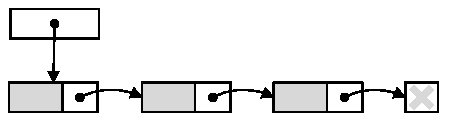
\includegraphics[width=\textwidth]{figures/collections/sll}
				\caption{Singly linked list}
				\label{fig:sll}
			\end{minipage}
			\hspace{0.5cm}
			\begin{minipage}[b]{0.45\linewidth}
				\centering
				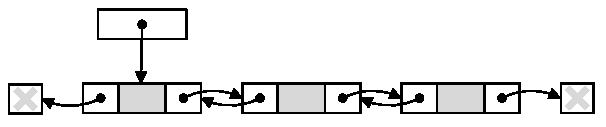
\includegraphics[width=\textwidth]{figures/collections/dll}
				\caption{Doubly linked list}
				\label{fig:dll}
			\end{minipage}
		\end{figure}
		\begin{figure}[h]
			\centering
			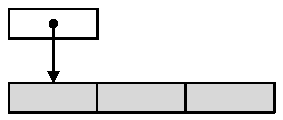
\includegraphics{figures/collections/list}
			\caption{Dynamic array or list structure}
			\label{fig:list}
		\end{figure}
		
		A variable number of nodes is implemented in an AST by nesting container nodes up to the depth required, forming either a singly-linked list (fig. \ref{fig:sll}) or a doubly-linked list (fig. \ref{fig:dll}). A node holding any number of child nodes might be represented in C\# as in snippet \ref{fig:col-sample}.
		
		\begin{lstlisting}[caption=Example of list attributes in a function definition,label=fig:col-sample]
class FunctionDefinition : Node 
{
	[Child] public List<VarDec> Variables { get; set; }
	[Child] public List<Statement> Statement { get; set; }
	[Child] public Expression Return { get; set; }
}
		\end{lstlisting}
	
		This poses the question how such a list should be treated. I should we see a list of nodes as a special type of node with no traversible children but traversible or can the functionality  \code{ChildAttribute} defined in section \ref{sec:type-safe-ast} 
		
		Case with collections:
		- Node child may be node (or derived) or list of nodes
		- Discriminated union in C\# (https://stackoverflow.com/questions/3151702/discriminated-union-in-c-sharp)
		- What doesn't work: Every node is also a list of nodes
		- Cyclic dependency in inheritance (Node : IList?)
		- Advantages: easy to add, iterate and replace
		- Disadvantages: Traversal issues (can a handler return a list?), complicates everything
		
		Case without collections:
		- More natural to traversals
		- Singly-linked or doubly-linked
		- Difficult to append to or modify
		- Can be overcome with extension methods
		
		Outcome: chosen for no collection types in lists, to avoid confusion with traversals.
			
	\section{Development Environment}
		Implications of unmanaged vs managed, reduction of base library, debug upgrade..?
		
		\subsection{Updated Lexer/Parser}
			More flexible Parser/Lexer generator support, such as ANTLR4 (LL(*) with EBNF).
						
			Language dependency: Plenty of parsers exist for any language, first version of AST most likely constructed in code; change of language not essential.
			
			Platform dependency: Depends on extensibility of parser generator, ANTLR4 has multiple ways of traversing a generated parse tree, YACC does not (embedding of code in parse phase restricts construction of AST)
			
		\subsection{Platform Updates}
			NuGet
			
		\subsection{Documentation Generator}
			Inheritance graph plotter, AST graph plotter
	
	\section{Validation}
		Type-safety is more than enough?
		
		Old method was not type safe, simply prevented untracable errors
		
		Tree corruption unnoticed until check routine ran
		
		Classes as f
	
\chapter{Discussion}
	vNext immutable AST, 
	
	Language choice, developers switch language often
		We found that developers rapidly and frequently learn
		languages. Factors such as age play a smaller role than suggested
		by media. In contrast, which languages developers
		learn is influenced by their education, and in particular, curriculum
		design.
		
	Functional
		Promisingly, developers who learned a functional or	math-oriented language in school are more than twice as likely to know one later than those who did not.

\bibliography{report}
\bibliographystyle{plainnat}
\end{document}